\documentclass[11pt]{article}
\usepackage[a4paper,margin=25mm]{geometry}
\usepackage{amsmath,amssymb,booktabs,hyperref,xcolor,graphicx,placeins}
\hypersetup{colorlinks=true,urlcolor=blue,citecolor=blue,linkcolor=blue}
\newcommand{\Rb}{R_b}
\newcommand{\VP}{F_{\mathrm{VP}}}
\title{Erratum to ``Hadronic cross section of $e^+e^-$ annihilation at bottomonium energy region''\\[3pt]\large Chinese Physics C \textbf{44}, 083001 (2020)}
\author{Xiang-Kun Dong, Xiao-Hu Mo, Ping Wang, and Chang-Zheng Yuan}
% \date{Draft for coauthor discussion --- 20 October 2026}
\begin{document}
\maketitle

In Ref.~\cite{original}, the charm-region input was described as the published inclusive $R$ measurements of the BES Collaboration. The calculation instead used, in part, an unpublished charm-region input. We correct this inconsistency by using the published BES measurements~\cite{bes2000,bes2002}: the $3.70$-$4.80\,\mathrm{GeV}$ points from Ref.~\cite{bes2002} and the $5.00\,\mathrm{GeV}$ point from Ref.~\cite{bes2000}.

The numerical review identified an omitted factor $1/\alpha(0)$ in the hadronic VP imaginary part, an incorrect conversion constant in the low-energy two-pion contribution, and insufficient control of the ISR iteration convergence. We have corrected these errors, improved the numerical evaluation of the VP principal-value integral, and removed the inconsistent additional smoothing before the VP calculation. The printed dispersion relation remains valid.

Figures~\ref{fig:cross} and \ref{fig:isr-vp} show the recalculated results with total propagated input uncertainties. Numerical data and their uncertainties are available in our GitHub repository~\cite{repository}.

\begin{figure}[htbp]\centering
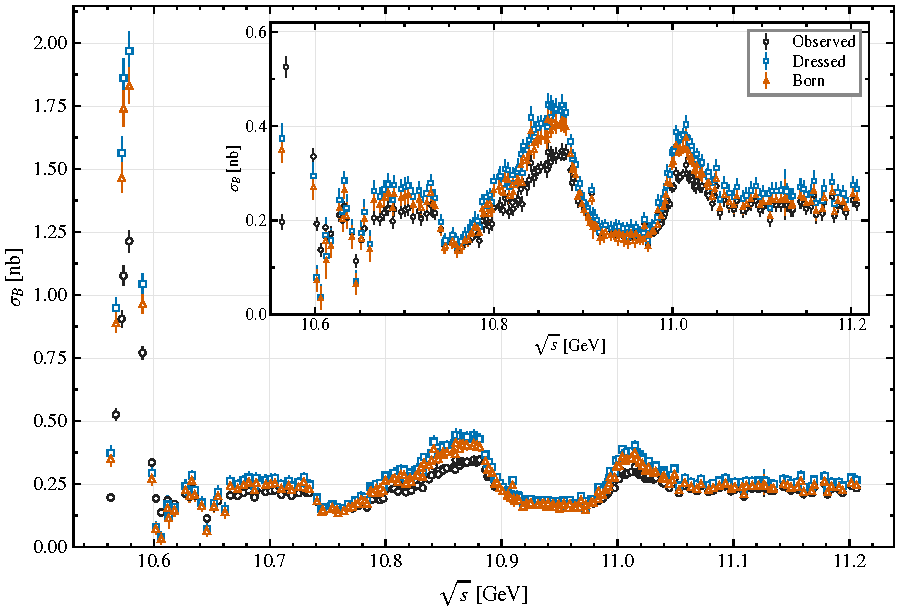
\includegraphics[width=.92\linewidth]{figures/cross_sections.pdf}
\caption{Observed, dressed, and Born cross sections at the 209 measured energies. Error bars show the propagated total input uncertainties. The observed points are the unsmoothed experimental input. The inset enlarges the region over $10.55$--$11.22\,\mathrm{GeV}$.}\label{fig:cross}
\end{figure}
\begin{figure}[t]\centering
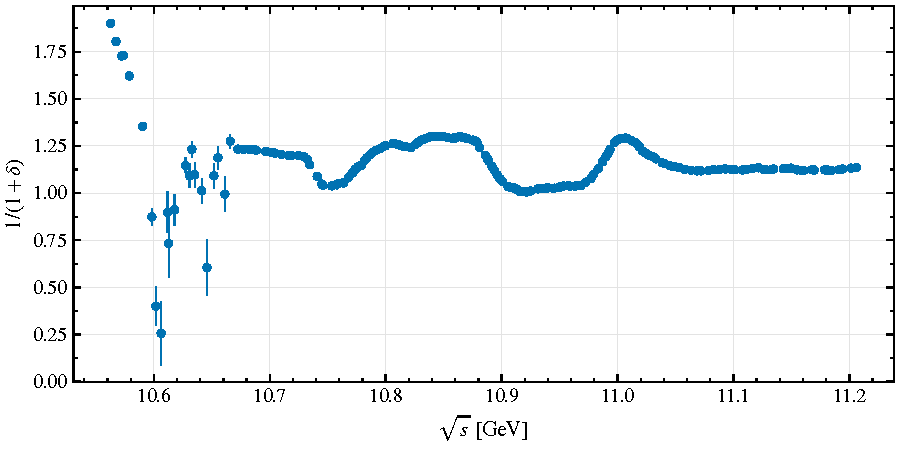
\includegraphics[width=.92\linewidth]{figures/isr.pdf}
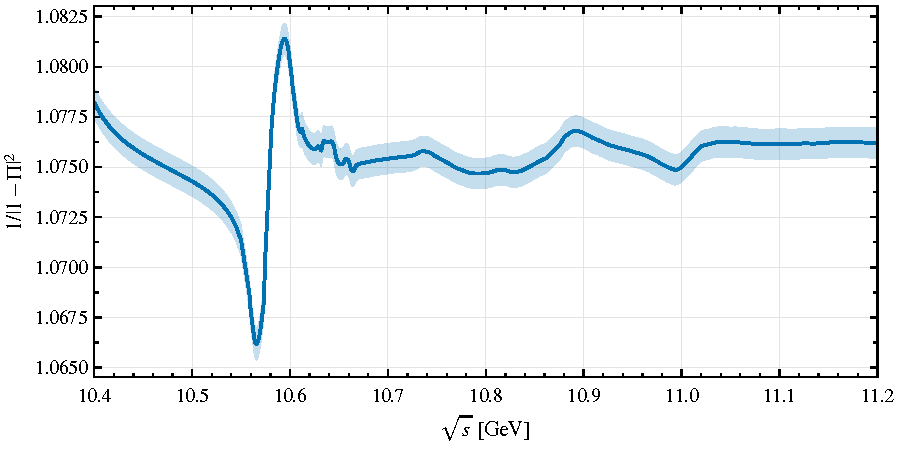
\includegraphics[width=.92\linewidth]{figures/vp.pdf}
\caption{Recalculated ISR correction factors (top) and VP factors (bottom). The error bars (top) and shaded band (bottom) show the propagated total input uncertainties.}\label{fig:isr-vp}
\end{figure}


% \FloatBarrier
\begin{thebibliography}{9}
\bibitem{original} X.-K. Dong, X.-H. Mo, P. Wang, and C.-Z. Yuan, Chinese Phys. C \textbf{44}, 083001 (2020), \href{https://doi.org/10.1088/1674-1137/44/8/083001}{doi:10.1088/1674-1137/44/8/083001}.
\bibitem{bes2000} J. Z. Bai et al. (BES Collaboration), Phys. Rev. Lett. \textbf{84}, 594 (2000), \href{https://doi.org/10.1103/PhysRevLett.84.594}{doi:10.1103/PhysRevLett.84.594}.
\bibitem{bes2002} J. Z. Bai et al. (BES Collaboration), Phys. Rev. Lett. \textbf{88}, 101802 (2002), \href{https://doi.org/10.1103/PhysRevLett.88.101802}{doi:10.1103/PhysRevLett.88.101802}.
\bibitem{repository} GitHub repository, \url{https://github.com/xkDong/VP-factors-at-bottomonium-region}.
\end{thebibliography}
\end{document}
